\chapter{鮮度の表現方法の検証}
\label{chap:verification}

本章では、情報の鮮度の視覚化について様々な視覚化の方法を試し、それぞれ考察していく。

以下で検証する全ての項目に関して図\ref{fig:ver_base}を利用する。

\begin{figure}[htbp]
  \begin{center}
    \fbox{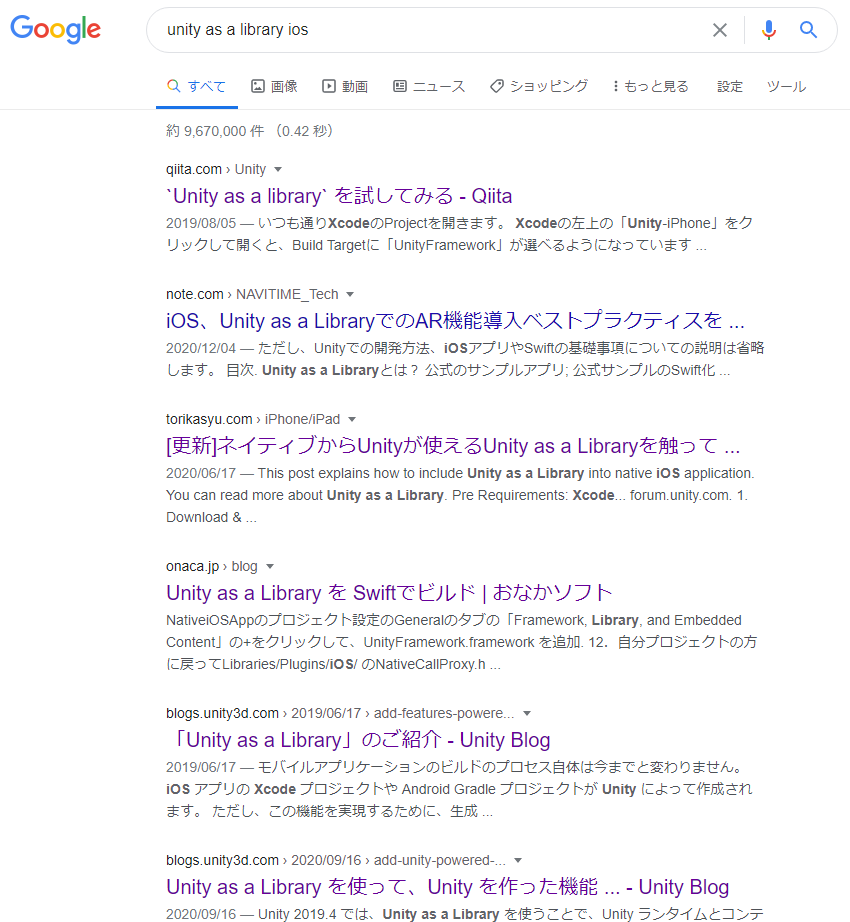
\includegraphics[width=60mm]{images/base.png}}
  \end{center}
  \caption{視覚化前の検索結果一覧}
  \label{fig:ver_base}
\end{figure}


\section{テクスチャによる変化}
\label{sec:ver_texture}

テクスチャを適用することで鮮度を視覚化する方法を検証する。

\subsection{紙の経年劣化}
\label{subsec:ver_tex_sheet}

実世界に存在する記録媒体で劣化するものを考えたときに最初に思い浮かんだのが紙である。

紙は時間が経つと黄ばみやシミができる。そういった変化を参考に、情報の鮮度を視覚化した。

\begin{figure}[htbp]
  \begin{minipage}{0.5\hsize}
    \begin{center}
      \fbox{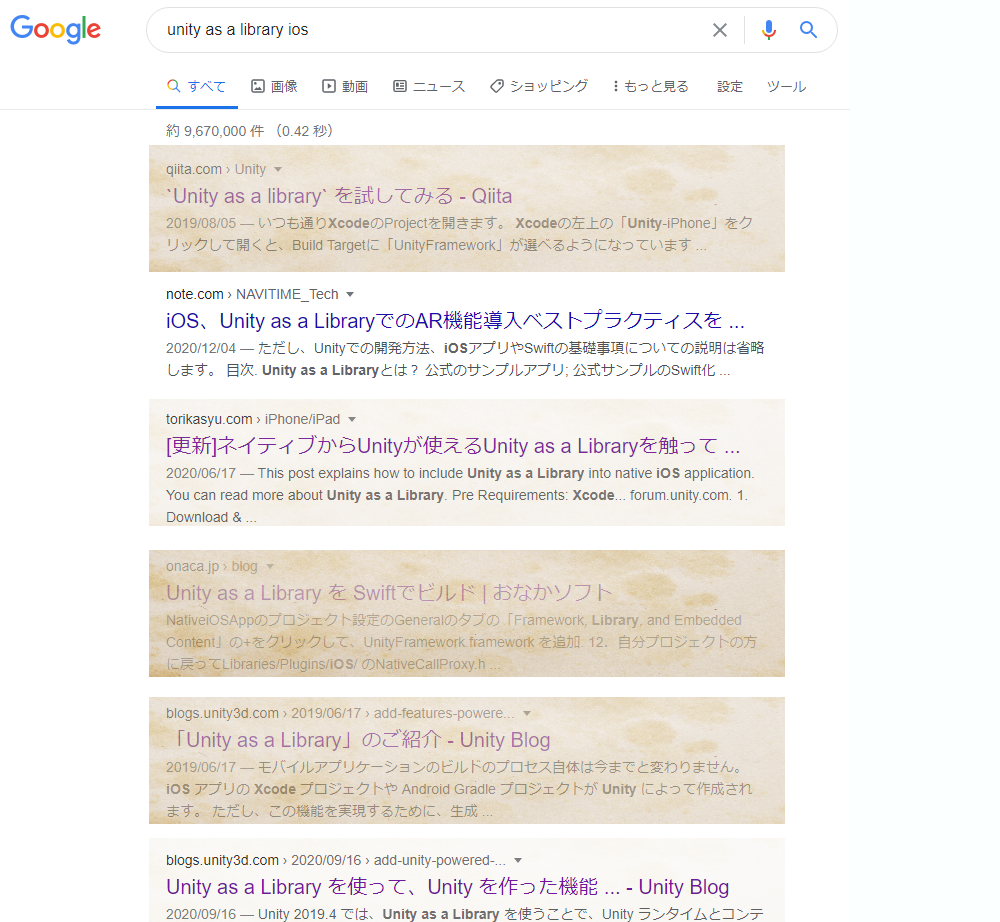
\includegraphics[width=60mm]{images/sheet-degradation1.png}}
    \end{center}
    \caption{紙の経年劣化をイメージした視覚化1}
    \label{fig:ver_sheet1}
  \end{minipage}
  \begin{minipage}{0.5\hsize}
    \begin{center}
      \fbox{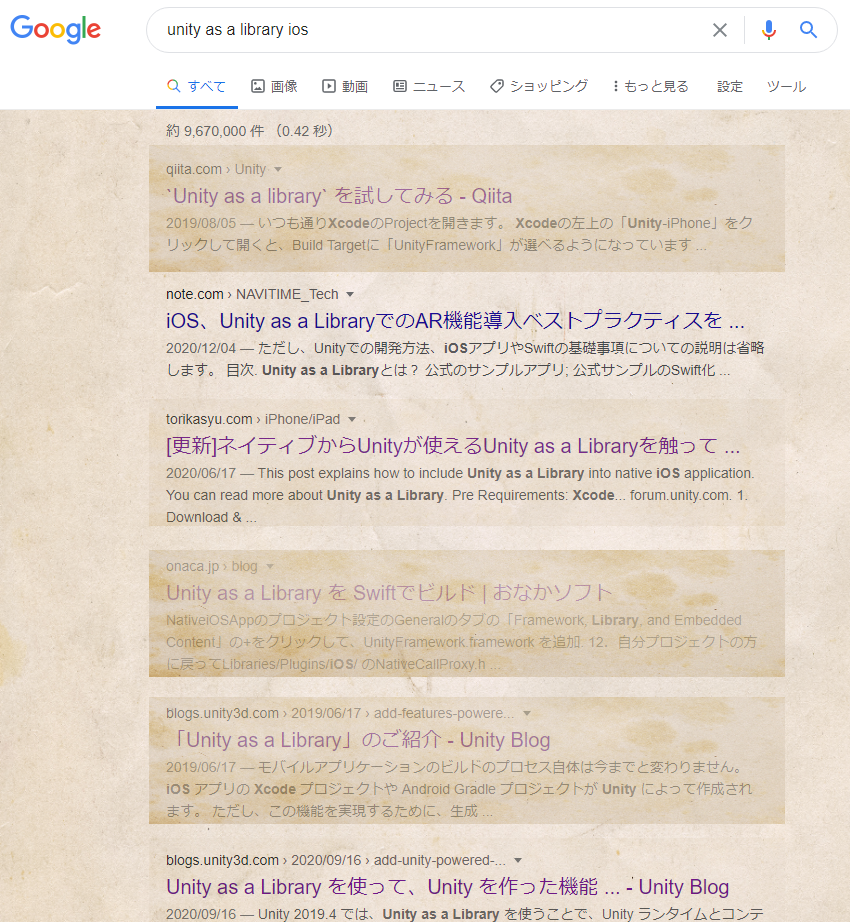
\includegraphics[width=60mm]{images/sheet-degradation2.png}}
    \end{center}
    \caption{紙の経年劣化をイメージした視覚化2}
    \label{fig:ver_sheet2}
  \end{minipage}
\end{figure}

各検索結果ごとに公開日を参考に、劣化した紙のテクスチャを適用したのが図\ref{fig:ver_sheet1}である。

さらに、全体に紙のテクスチャを適用することで劣化した紙のテクスチャが背景になじむように調整したのが図\ref{fig:ver_sheet2}である。

紙の劣化を参考にしているためか、古いということが分かりやすい。家や図書館などで古くなった本を見た経験がある人ならば、紙の時間経過による劣化を連想しやすいのではないだろうか。

図\ref{fig:ver_sheet1}に比べて、図\ref{fig:ver_sheet2}の方が背景に紙のテクスチャを設定しているため劣化した紙のテクスチャに違和感が少ない。

\subsection{金属のさび}
\label{subsec:ver_tex_russet}

実世界に存在するモノで紙以外に外見的な劣化の参考になるものを考えたとき、次に浮かんだのは金属である。

金属は雨風にさらされることでさびが発生するため、時間経過による劣化が簡単に見て取れる。これを参考に視覚化を行った。

\begin{figure}[htbp]
  \begin{minipage}{0.5\hsize}
    \begin{center}
      \fbox{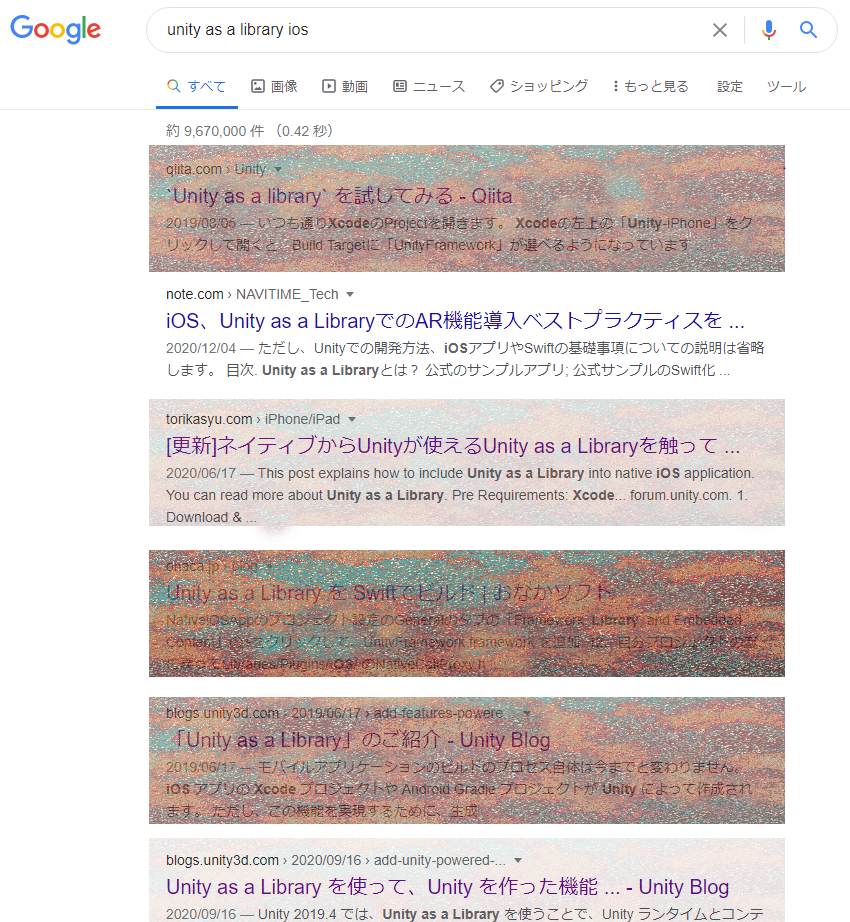
\includegraphics[width=60mm]{images/iron-russet1.png}}
    \end{center}
    \caption{金属のさびをイメージした視覚化1}
    \label{fig:ver_russet1}
  \end{minipage}
  \begin{minipage}{0.5\hsize}
    \begin{center}
      \fbox{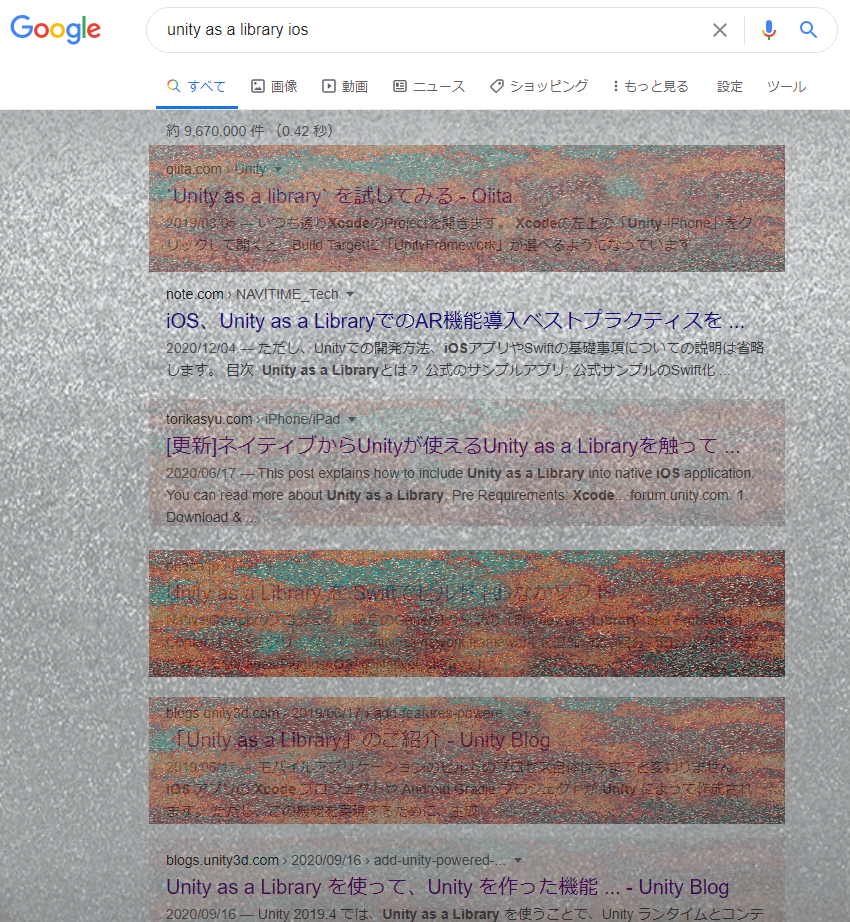
\includegraphics[width=60mm]{images/iron-russet2.png}}
    \end{center}
    \caption{金属のさびをイメージした視覚化2}
    \label{fig:ver_russet2}
  \end{minipage}
\end{figure}

\ref{subsec:ver_tex_sheet}の方法と同様に、錆びた金属のテクスチャを適用したのが図\ref{fig:ver_russet1}である。

また、背景に錆びていない金属のテクスチャを適用したのが図\ref{fig:ver_russet2}である。

\ref{subsec:ver_tex_sheet}と比べて古い情報が強調されているが、背景に金属のテクスチャを適用してもぬぐい切れない不自然さがある。

文字が記録されている媒体として金属があまり適していないことが原因と推測される。

\section{色による変化}
\label{sec:ver_color}

背景色や文字色を変更することで鮮度を視覚化する方法を検証する。

\subsection{背景の色褪せ}
\label{subsec:ver_col_cor}

実世界のモノが腐食するイメージを参考に、背景の色褪せによって情報の鮮度を視覚化した。

\begin{figure}[htbp]
  \begin{minipage}{0.5\hsize}
    \begin{center}
      \fbox{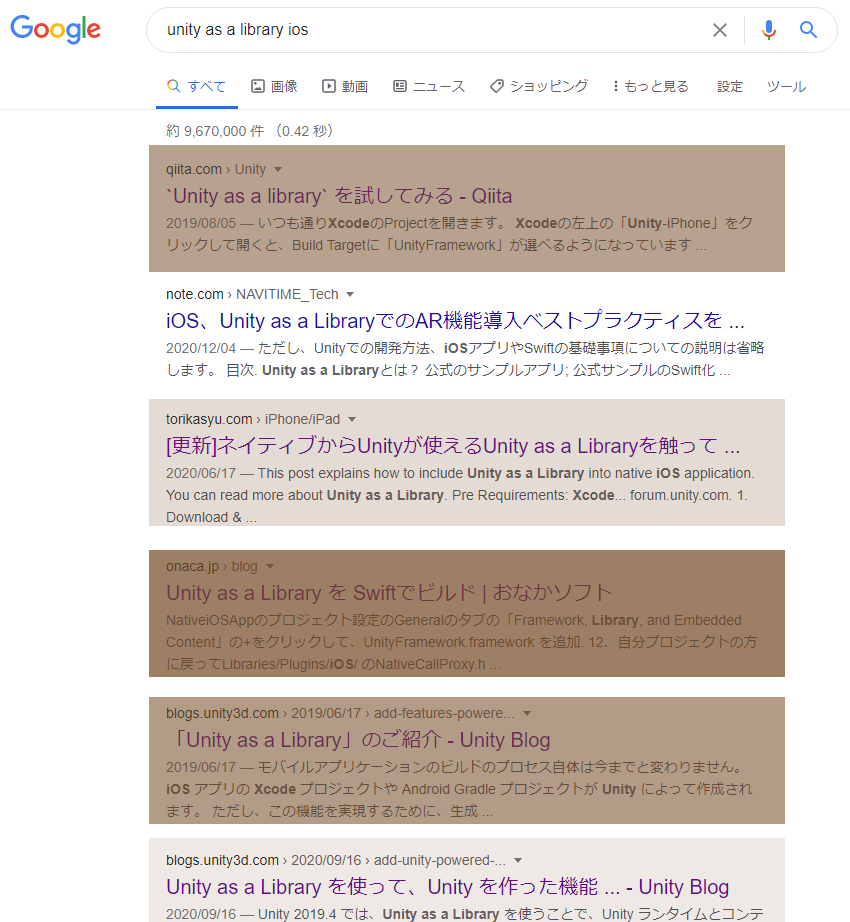
\includegraphics[width=60mm]{images/corrosion1.png}}
    \end{center}
    \caption{腐食をイメージした視覚化1}
    \label{fig:ver_corrosion1}
  \end{minipage}
  \begin{minipage}{0.5\hsize}
    \begin{center}
      \fbox{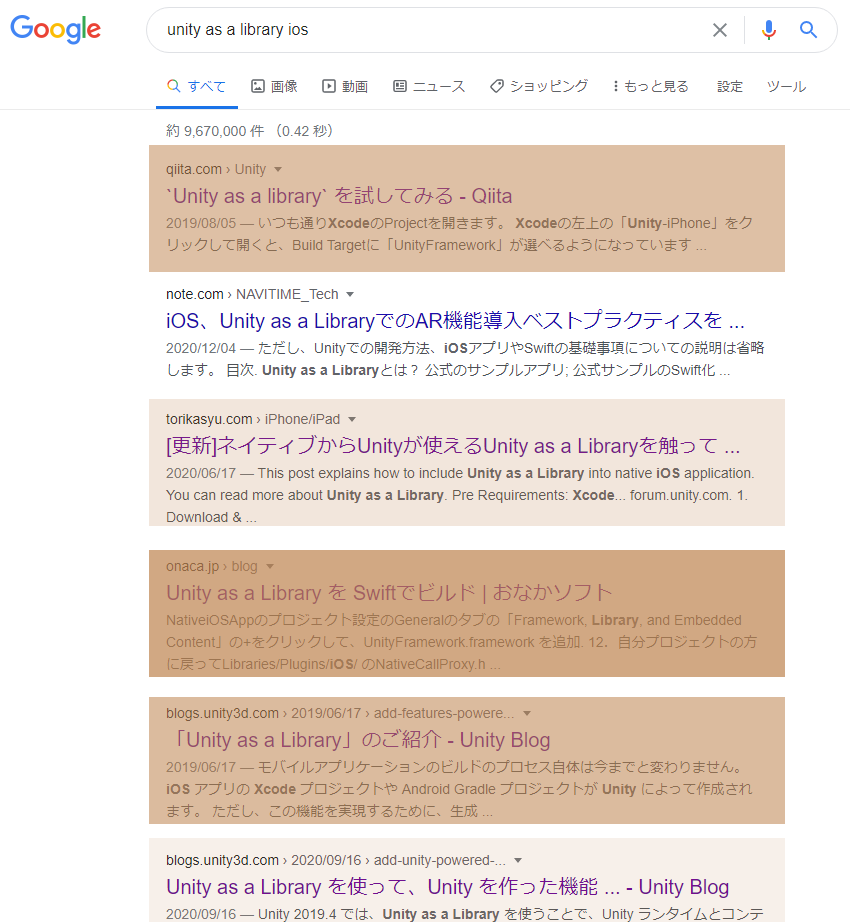
\includegraphics[width=60mm]{images/corrosion2.png}}
    \end{center}
    \caption{腐食をイメージした視覚化2}
    \label{fig:ver_corrosion2}
  \end{minipage}
\end{figure}

腐食を参考にしたため暗い茶色(図\ref{fig:ver_corrosion1})や赤茶色(図\ref{fig:ver_corrosion2})の中で鮮度ごとに色が変化するように、視覚化を適用している。

コンセプトとしては\ref{sec:ver_texture}で検証した二つと近いが、こちらの方がシンプルな分、元の白い背景に対して不自然さがないが、鮮度を示すものということが認識しにくい。

色の選定部分においては議論の余地があると考えられる。

\subsection{インクの劣化}
\label{subsec:ver_col_ink}

紙に書いた文字のインクが時間経過によって劣化していくのを参考に、情報の鮮度を視覚化した。

\begin{figure}[htbp]
  \begin{minipage}{0.5\hsize}
    \begin{center}
      \fbox{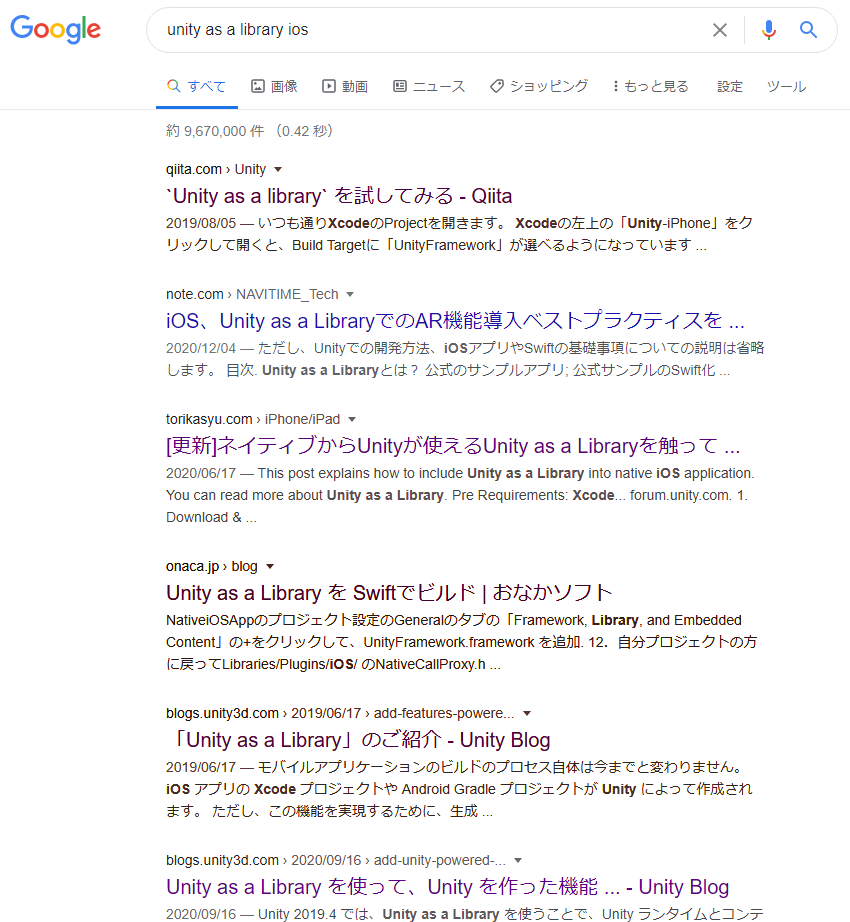
\includegraphics[width=60mm]{images/ink1.png}}
    \end{center}
    \caption{インクの劣化をイメージした視覚化1}
    \label{fig:ver_ink1}
  \end{minipage}
  \begin{minipage}{0.5\hsize}
    \begin{center}
      \fbox{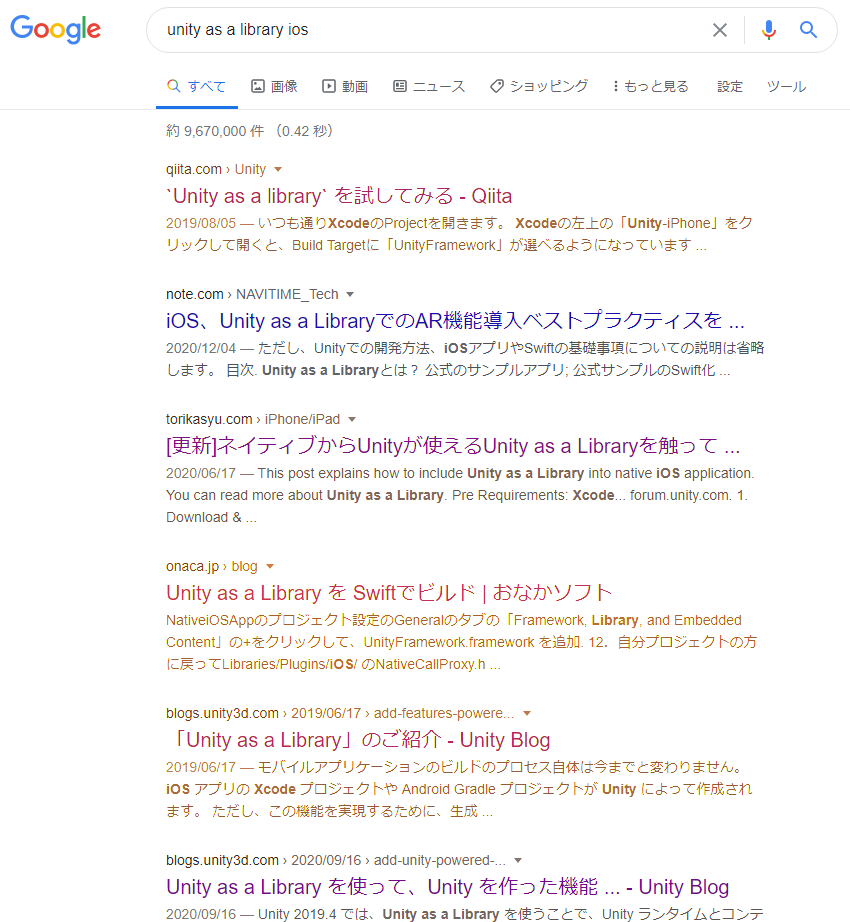
\includegraphics[width=60mm]{images/ink2.png}}
    \end{center}
    \caption{インクの劣化をイメージした視覚化2}
    \label{fig:ver_ink2}
  \end{minipage}
\end{figure}

\ref{subsec:ver_col_cor}と同様に、情報の鮮度に応じて文字の色が焦げ茶色に近づくようにしたのが図\ref{fig:ver_ink1}である。

また、背景色の白に薄まるように変化を加えたのが図\ref{fig:ver_ink2}である。

図\ref{fig:ver_ink1}に関しては、視覚化による変化が目立っておらずユーザに情報の鮮度を認識させるという目的が果たせていない。

図\ref{fig:ver_ink2}は、古い印象を与えることには成功しているが、古いか新しいかの二択に捉えられやすいと思われる。

どちらの場合も段階的な変化を認識しやすい視覚化の方法とは言えない。

\section{文字の消失による変化}
\label{sec:ver_character}

文字の一部、または全体を欠落させたり存在感を薄めることで鮮度を視覚化する方法を検証する。

\subsection{透明化}
\label{subsec:ver_chr_trp}

実世界のモノが時間経過によって消失していくさまをイメージして、各項目の不透明度を変更することで鮮度の視覚化を行った。

\begin{figure}[htbp]
  \begin{center}
    \fbox{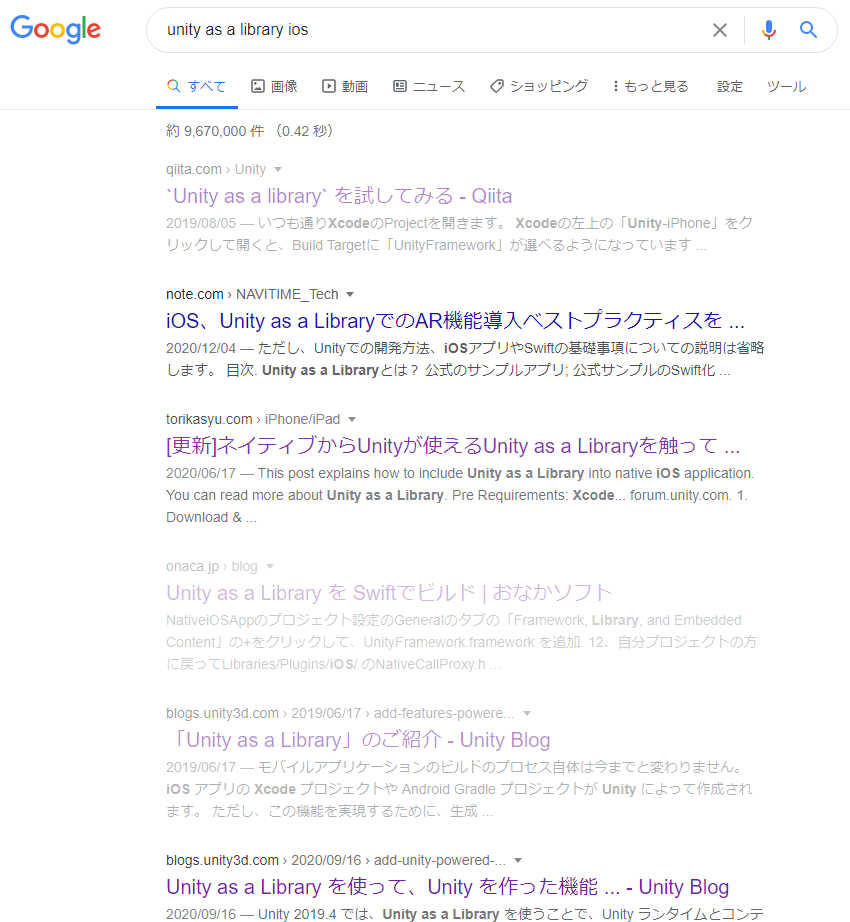
\includegraphics[width=60mm]{images/transparence.png}}
  \end{center}
  \caption{不透明度を変更した視覚化}
  \label{fig:ver_transparence}
\end{figure}

図\ref{fig:ver_transparence}は、各情報ごとに古いければ古いほど不透明度が下がっていくように視覚化を行ったものである。

元の検索画面に対して微小な変更のみを加えているため、不自然な点が少ない。また、段階的な変化が認識しやすく時間経過を簡単に見て取れる。

しかし薄いもの(不透明度が低いもの)が古いという結びつけが弱いため、鮮度を表しているという認識を与えられるか疑問がある。

\subsection{滲む}
\label{subsec:ver_chr_bld}

紙にインクをたらしたときにインクが滲んでいくイメージを参考に、鮮度を視覚化した。

\begin{figure}[htbp]
  \begin{center}
    \fbox{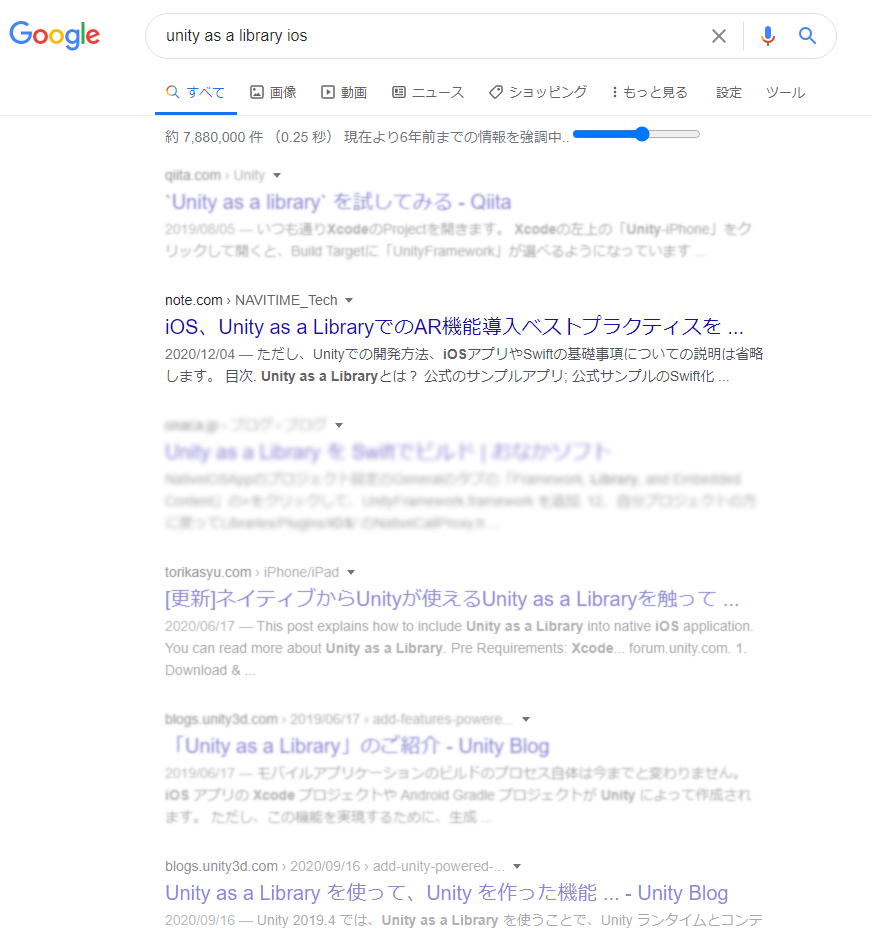
\includegraphics[width=60mm]{images/bleeding.png}}
  \end{center}
  \caption{インクの滲みをイメージした視覚化}
  \label{fig:ver_bleeding}
\end{figure}

\ref{subsec:ver_chr_trp}と同様の基準で、文字が滲むように変更を加えたのが図\ref{fig:ver_bleeding}である。

透明化のように元の背景とよくなじみ、段階的な変化が感じやすい。加えて、古いものを読ませないという効果も期待できる。

しかしながら、やはり滲んでいるから古い情報だという結びつけは弱いのではないだろうか。

\subsection{虫食い}
\label{subsec:ver_chr_wh}

古い書物などは紙自体の経年劣化の他にシミなどの虫による欠落が見られる。そういった劣化の仕方を参考に鮮度を視覚化した。

\begin{figure}[htbp]
  \begin{minipage}{0.5\hsize}
    \begin{center}
      \fbox{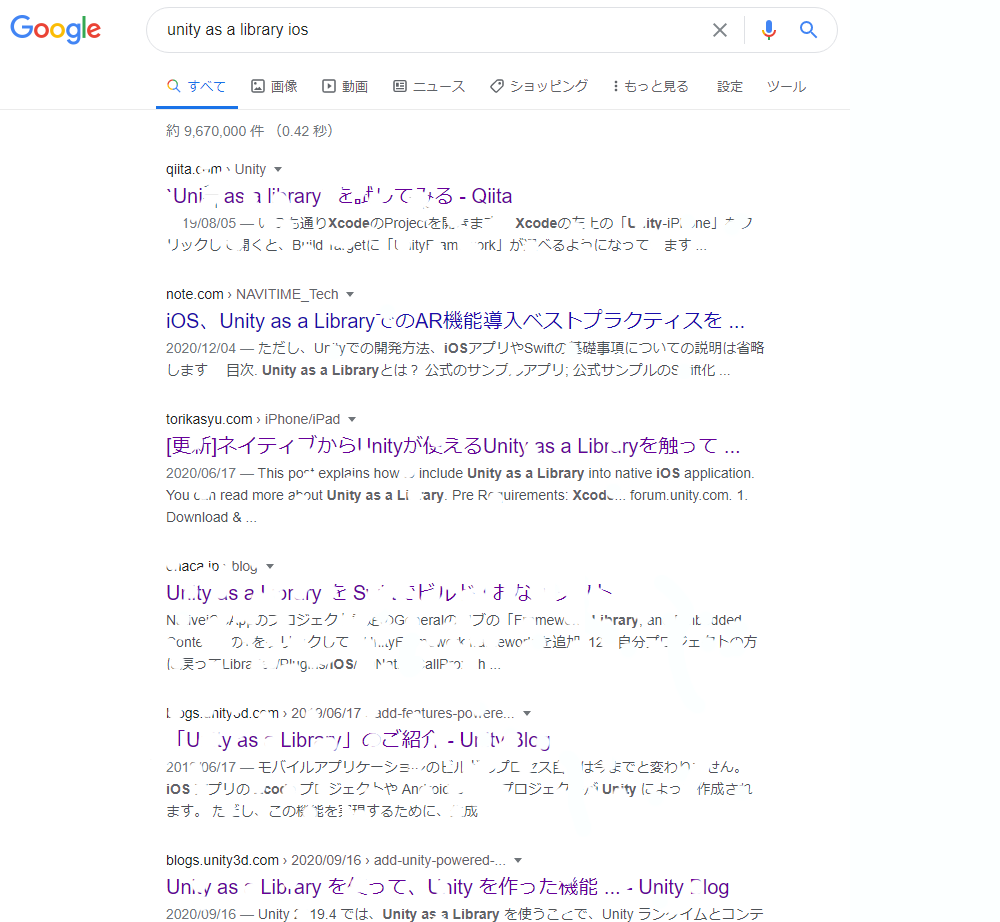
\includegraphics[width=60mm]{images/wormhole1.png}}
    \end{center}
    \caption{虫食いをイメージした視覚化1}
    \label{fig:ver_wormhole1}
  \end{minipage}
  \begin{minipage}{0.5\hsize}
    \begin{center}
      \fbox{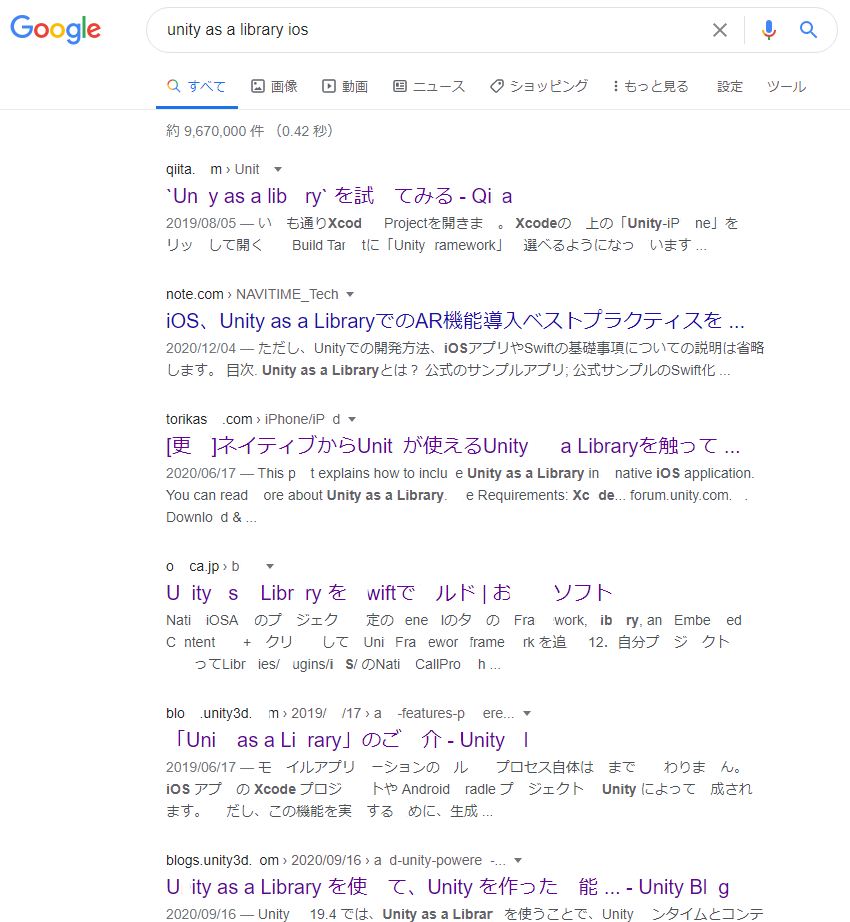
\includegraphics[width=60mm]{images/wormhole2.png}}
    \end{center}
    \caption{虫食いをイメージした視覚化2}
    \label{fig:ver_wormhole2}
  \end{minipage}
\end{figure}

図\ref{fig:ver_wormhole1}は実際に虫に食われた紙をイメージして、古いものがより欠損するように視覚化を行ったものである。

そして図\ref{fig:ver_wormhole2}は文章の虫食いをイメージして、古ければ古いほど多くの文字が欠落するように視覚化を行ったものである。

どちらも情報の鮮度に応じた変化の程度の差を設けるのが難しいが、古いものを読ませない効果は十分にあるだろう。

しかし、ある程度の文字が欠損していても何となくで読めてしまう部分があり、\ref{subsec:ver_col_ink}の視覚化と同様、段階的な変化ではなく読めるか読めないかの二分された認識になった。

\section{フォントによる変化}
\label{sec:ver_font}

使用されるフォントを変更することで鮮度を視覚化する方法を検証する。

\subsection{書体}
\label{subsec:ver_fnt_stl}

時代が進むごとに文字の書体も変わってきた\footnote{5分で学ぶフォントの歴史500年|時代背景とタイポグラフィ, https://note.com/smartcamp_design/n/n2740a3b72be9}。

古い情報は古そうだと感じられる書体を、新しい情報は新しそうだと感じられる書体を用いて記述することで情報の鮮度を視覚化した。

\begin{figure}[htbp]
  \begin{center}
    \fbox{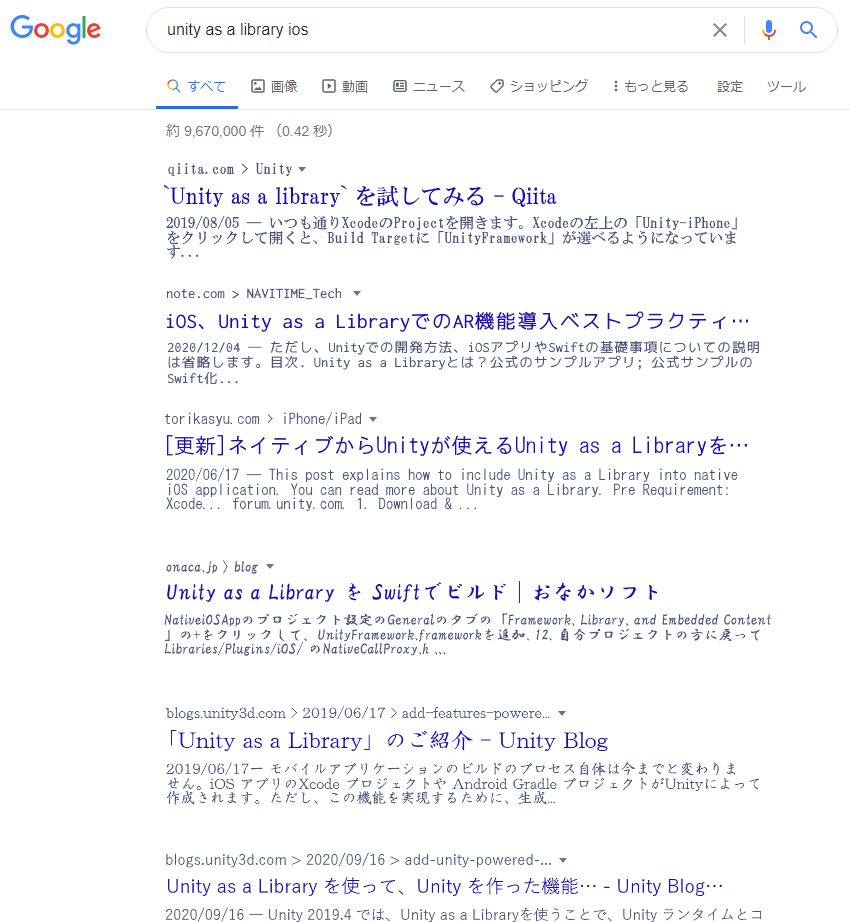
\includegraphics[width=60mm]{images/font-style.png}}
  \end{center}
  \caption{書体の変化による視覚化}
  \label{fig:ver_style}
\end{figure}

図\ref{fig:ver_style}は各情報ごとにWindowsに標準で搭載されているフォントを用いて、鮮度を視覚化したものである。

検証して分かったことだが、フォントの選定が難しく、人によって感じる印象が違うため鮮度を表すものとしては適さないと考えられる。

\subsection{ドット文字}
\label{subsec:ver_fnt_dot}

古い電子機器の画面ではピクセル数の関係からドット文字が使用されていたり、古さを演出するために意図的にドット文字を使うこともある。

そこで粒度の違うドット文字を用いて情報の鮮度を視覚化した。

\begin{figure}[htbp]
  \begin{center}
    \fbox{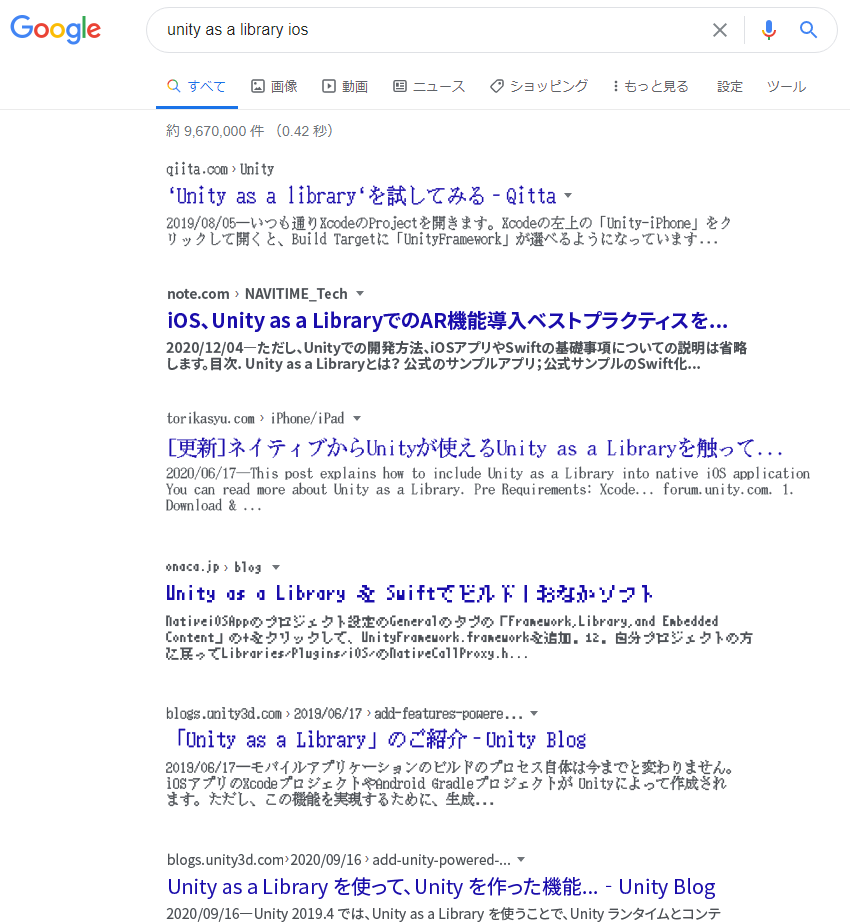
\includegraphics[width=60mm]{images/font-dot.png}}
  \end{center}
  \caption{ドット文字の粒度の変化による視覚化}
  \label{fig:ver_dot}
\end{figure}

古ければ古いほど粒度の荒いドット文字を使って表現したのが図\ref{fig:ver_dot}である。

予測では鮮度の段階ごとの変化を感じやすいと思われたが、古い印象よりも各サイトごとの特色だという印象の方が強かった。

これは各ドット文字がそれぞれ特徴的で、段階的な変化を感じさせなかったためだと推測される。

\section{その他の変化}
\label{sec:ver_other}

以上までに分類されない変化を用いて鮮度を視覚化する方法を検証する。

\subsection{テロメア}
\label{subsec:ver_oth_tlm}

Scrapboxというサービス\footnote{https://scrapbox.io/}内で用いられている、更新時刻を視覚化する機能\footnote{https://scrapbox.io/shokai/%E3%83%86%E3%83%AD%E3%83%A1%E3%82%A2}を参考に情報の鮮度の視覚化を行った。

\begin{figure}[htbp]
  \begin{center}
    \fbox{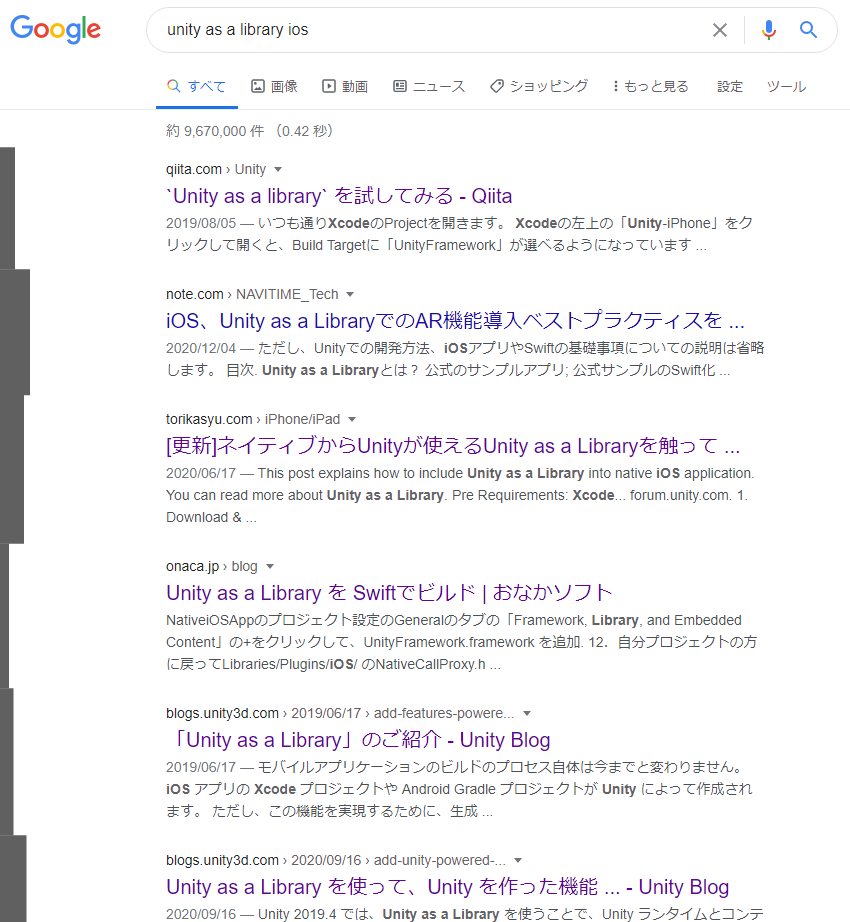
\includegraphics[width=60mm]{images/telomere.png}}
  \end{center}
  \caption{テロメアによる視覚化}
  \label{fig:ver_telomere}
\end{figure}

図\ref{fig:ver_telomere}は画面左端にテロメアを適用したものである。

各情報の鮮度ごとの段階的な変化が分かりやすく、それぞれの程度の差も直感的に感じられる。

しかし、同サービスを利用した経験がないユーザにはこれが情報の鮮度を表したものだと認識しにくいのではと推測される。

